\documentclass[10pt,a4paper]{article} % font size + paper
\usepackage[margin=2cm]{geometry} % setting up geometry
\usepackage{graphicx}
\usepackage{helvet} % using helvetica-like font
\usepackage[colorlinks=false]{hyperref} % for links
% for the content
\usepackage{array, xcolor}
\definecolor{lightgray}{gray}{0.8}
\newcolumntype{L}{>{\raggedleft}p{0.14\textwidth}}
\newcolumntype{R}{p{0.8\textwidth}}
\newcommand\VRule{\color{lightgray}\vrule width 0.5pt}
\usepackage{natbib}
\usepackage{bibentry}
\usepackage{tikz}

%%% Example how to add content %%%

%\section*{Heading}
% \begin{tabular}{L!{\VRule}R}
%  2012&Some text\\[5pt]
%  2011&Some other text\\
% \end{tabular}

% for try out
%\usepackage{lipsum}

% headers
\usepackage{fancyhdr}
\pagestyle{fancy}
\rfoot{Barcelona, Spain}
\lfoot{\today}
\renewcommand{\headrulewidth}{0pt}
\renewcommand{\footrulewidth}{0pt}

% name
\title{\bfseries\huge David Mas-Ponte}
% Job
\author{Bioinformatics - Genome instability }
% today's date
\date{}

% fonts
 \renewcommand{\familydefault}{\sfdefault}

%img path
\graphicspath{{img/}}

\begin{document}

% Header
% should be 0.65 if adding the picture below
\begin{minipage}[c]{\textwidth}
% make title puts the name and mail in the left
\maketitle
\end{minipage}
%\begin{minipage}[c]{0.3\textwidth}
%profile picture
%  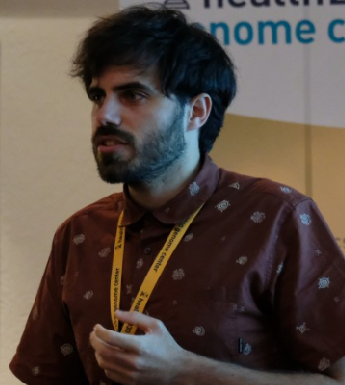
\includegraphics[width=.55\textwidth]{profile}
%\end{minipage}


% Subheader
\begin{minipage}[c]{0.5\textwidth}
  \begin{center}
    \href{mailto:david.mas.p@gmail.com}{david.mas.p@gmail.com}\\
    Barcelona, Spain
  \end{center}
\end{minipage}
\begin{minipage}[c]{0.5\textwidth}
  \begin{center}
\href{https://github.com/davidmasp}{github://davidmasp}

\includegraphics[height=12pt]{gh}\\
\href{http://david.masponte.com/}{david.masponte.com}
\end{center}
\end{minipage}

\vspace{0.5cm}
\rule{.95\textwidth}{0.75pt}

%%%% EDUCATION %%%%

\renewcommand{\arraystretch}{0.7} 

\section*{Education}
\begin{tabular}{L!{\VRule}R}
  2017--2022&{\bf Ph.D. in Biomedicine}\\
  & Universitat de Barcelona, Barcelona, Spain.\\
  & {\em \color{black!50} Current }\\[15pt]
  2015--2017& M.Sc. in Bioinformatics for Health Sciences\\
   & Universitat Pompeu Fabra, Barcelona, Spain.\\
   & {\em \color{black!50} Specialization in Genomics - GPA: 9 / 10 }\\[15pt]
  2011--2015&B.Sc. in Biotechnology\\
   & Universitat Autonoma de Barcelona, Spain.\\
   & International exchange (6 months), McGill University, Montreal, Canada\\
   & { \em \color{black!50} GPA: 8.5 / 10}
\end{tabular}

\renewcommand{\arraystretch}{1.5} 

%%%% Research %%%%
\section*{Research Experience}
\begin{tabular}{L!{\VRule}R}
01 2022 - &{\bf Stanford University } - {\em \color{black!70} Visiting Student Researcher }   \\
 & As part of my Ph.D. research I am visiting the laboratory of Ashby Morrison where
I study the susceptibility of DNA to UV dammage in human cell lines and tissues.
I am analysing a comprehensive dataset of genomic and epigenomic data to quantify
 the role of UV damage in the determination of somatic mutation rates. {\bf Ashby Morrison's Lab} \\
08 2017 -  &{\bf Institute for Research in Biomedicine } - {\em \color{black!70} Ph.D. Student }   \\
 & In my Ph.D. project, I study how somatic mutations accumulate in the genome of both
 tumor and healthy cells.
  We use statistical and machine learning techniques to extract patterns or {\em signatures}
  from available sequencing data sets. We are particularly interested in unraveling 
  mechanisms of local variability in mutation rates, such as the mutation clusters generated 
  by the APOBEC3 gene family and the effects of epigenetic features on DNA. {\bf Fran Supek's Lab}\\
2016 - 2017&{\bf Centre for Genomic Regulation (CRG) } - {\em \color{black!70} Master Science Research Thesis  }\\
 & During my master thesis I studied the link between lncRNAs' 
 subcellular localization and their function. I characterized 
 the associated variability and systematically compared against 
 protein coding genes. I also developed a web-based application 
 to make subcellular expression data of lncRNAs available to the
  scientific community. {\bf Roderic Guigo's Lab, tutored by Rory Johnson}\\
2015-2016 & {\bf Institute of Evolutionary Biology (IBE) } - {\em \color{black!70} Part time Research Internship}\\
 & During the first year of my master's program, I participated in the generation
 and analysis of sequencing data to study the demographic and adaptive processes shaping the RhD blood group
  system in the Basque population. {\bf David Comas' Lab}\\[15pt]
\end{tabular}

\vspace{10pt}

%%%% Programing %%%%

%%%% pubs %%%%
\renewcommand{\arraystretch}{1.5} 
\bibliographystyle{unsrtnat}
\nobibliography{dmas}

\section*{Selected Publications} 

Find a complete list at \href{https://orcid.org/0000-0001-7409-305X}{orcid.org/0000-0001-7409-305X}.
Lead author publications highlighted with * .
\\
\\
% if you remove the \textbf{} it breaks
\begin{tabular}{L!{\VRule}R}
2022 &\textbf{} * \bibentry{mas-ponte_spectrum_2022} - {\em \color{black!70} Review article} \\
2020 &\textbf{} * \bibentry{mas_dna_2020} - {\em \color{black!70} Peer-reviewed}\\
2019 &\textbf{} \bibentry{franco_whole_2019} - {\em \color{black!70} Peer-reviewed} \\
2018 &\textbf{} \bibentry{flores-bello_sequence_2018} - {\em \color{black!70} Peer-reviewed} \\[30pt]
2017 &\textbf{} * \bibentry{mas-ponte_lncatlas_2017} - {\em \color{black!70} Peer-reviewed}\\[5pt]
\end{tabular}


\section*{Selected Conferences}

\begin{tabular}{L!{\VRule}R}
2021 &\textbf{}\bibentry{mas_EACR_2021} - {\em \color{black!70} Peer-reviewed Conference - Short talk} \\[30pt]
2019 &\textbf{}\bibentry{david_mas-ponte_hypermut_2019} - {\em \color{black!70} Peer-reviewed Conference - Poster} \\[30pt]
2018 &\textbf{}\bibentry{david_mas-ponte_association_2018} - {\em \color{black!70} Peer-reviewed Conference - Poster} \\
\end{tabular}

%%%% SA %%%%
\section*{Other scientific contributions \& Awards}

\renewcommand{\arraystretch}{1} 

\begin{tabular}{L!{\VRule}R}
2021 & \textbf{SCB award to the best scientific article} -  {\em \color{black!70} Nominee}   \\
& The \textit{Societat Catalana de Biologia} (SCB) is the society that groups all professional and academic biologist
in Catalonia. Every year, they award a recognition to the best scientific article in life sciences published in an international journal. In 2021, my paper (\textit{Mas-Ponte Nature Genetics 2020}) got selected as one of the nominees for this award \\[60pt]
2018-2019 & \textbf{ENABLE 2019} -  {\em \color{black!70} Scientific Organizing Committee}   \\
& ENABLE is an international scientific conference for Ph.D. Students from all over the world co-organized by 4 European research centers (IRB Barcelona, RIMLS, CPR, and SEMM) funded by the European Union Horizon 2020 program. The third edition was held in the city of Nijmegen in the Netherlands with a total of 229 Ph.D. students and postdocs coming from 26 different countries.
 \end{tabular}

 \clearpage

%%%% SA %%%%
\section*{Working papers}

This section contains abstracts for manuscripts currently in preparation.

\bigskip

\begin{tabular}{L!{\VRule}R}
2022 & \textbf{Variable DNA methylation underlies mutation rate variability at the mesoscale in human somatic cells} -  {\em \color{black!70} Manuscript in preparation}   \\
& 

\bigskip

\textbf{Abstract}:



The cytosine methylation in CpG dinucleotides is pervasive in mammalian genomes and its variability across regions can regulate gene expression and define cell differentiation. Although the role of DNA methylation in gene regulation is well understood, how the local variation in DNA methylation shapes somatic mutation rates is less well explored. Here, we show that hypomethylated (UMR) regions are also generally hypomutated in a wide range of human tumors and healthy somatic tissues.

\medskip

Remarkably, the exposure of the tissue to various mutational processes shapes its predisposition to this effect: while there is depletion in the mutation rates resulting from signatures of deamination of methylated cytosines, UV light, POLE and MMR deficiency, there is an increase in mutation rates from signatures of AID/APOBEC cytosine deaminase enzymes in the UMRs. Therefore, hypomethylated DNA loci can be either mutational coldspots or hotspots, depending on the mutagen exposure history of a particular cell.

\medskip

In addition to these genome-wide distributed UMRs we also identify several kilobases at the 5’ ends of gene bodies as commonly hypomethylated and thus hypomutated. Clustering genes by methylation profiles also yielded variability in their mutation rate gradients along the gene body. Interestingly, lowly expressed genes have a less steep gradient due to a higher relative methylation of their 5’ end, and polycomb repressed genes also show no relative hypomutation due to the lack of methylation at their gene body.


\medskip


Overall, we suggest DNA methylation is an important determinant of mesoscale, sub-genic, resolution mutation rate variability in human somatic tissues.


\end{tabular}

\end{document}
